\chapter{Pseudorandom functions from pseudorandom
generators}\label{Pseudorandom-functions-fr}

We have seen that PRF's (pseudorandom functions) are extremely useful,
and we'll see some more applications of them later on. But are they
perhaps too amazing to exist? Why would someone imagine that such a
wonderful object is feasible? The answer is the following theorem:

\hypertarget{prfthm}{}
\begin{theorem}[The PRF Theorem] \label[theorem]{prfthm}

Suppose that the PRG Conjecture is true, then there exists a secure PRF
collection \(\{ f_s \}_{s\in\{0,1\}^*}\) such that for every
\(s\in\{0,1\}^n\), \(f_s\) maps \(\{0,1\}^n\) to \(\{0,1\}^n\).

\end{theorem}


\begin{figure}
\centering
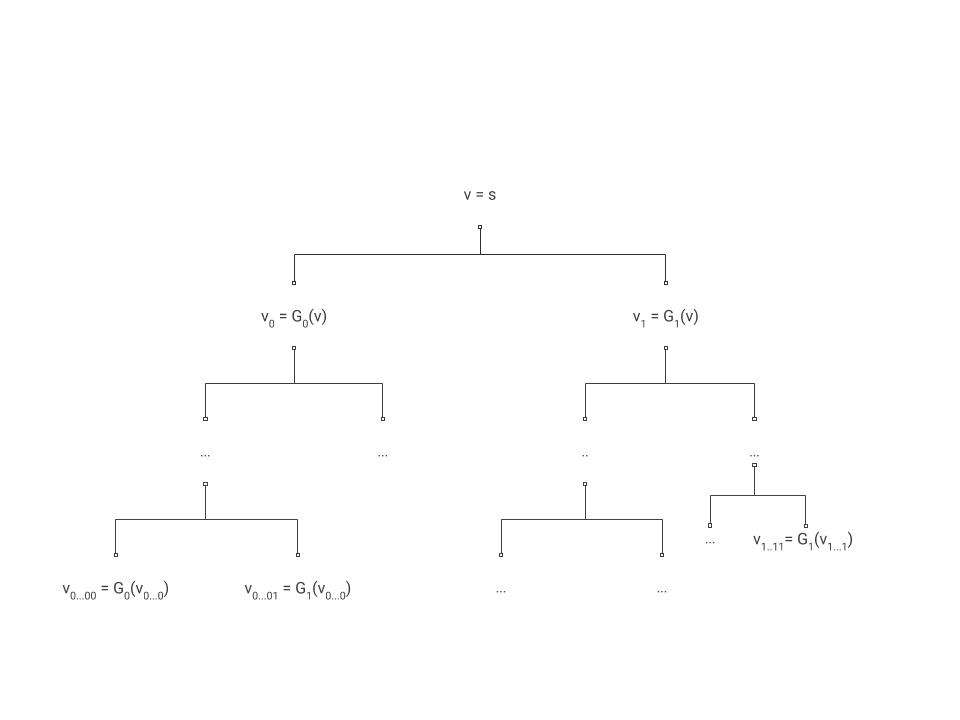
\includegraphics[width=\textwidth, height=0.25\paperheight, keepaspectratio]{../figure/PRF_from_PRG.jpg}
\caption{The construction of a pseudorandom function from a pseudorandom
generator can be illustrated by a depth \(n\) binary tree. The root is
labeled by the seed \(s\) and for every internal node \(v\) labeled by a
strong \(x\in\{0,1\}^n\), we use that label \(x\) as a seed into the PRG
\(G\) to label \(v\)'s two children. In particular, the children of
\(v\) are labeled with \(G_0(x)\) and \(G_1(x)\) respectively. The
output of the function \(f_s\) on input \(i\) is the label of the
\(i^{th}\) leaf counting from left to right. Note that the numbering of
leaf \(i\) is related to the bitstring representation of \(i\) and the
path leaf \(i\) in the following way: we traverse to leaf \(i\) from the
root by reading off the \(n\) bits of \(i\) left to right and descend
into the left child of the current node for every 0 we encounter and
traverse right for every 1.}
\label{PRFfromPRGfig}
\end{figure}

\begin{proof} \label[proof]{If-the-PRG-Conjecture-is-}

If the PRG Conjecture is true then in particular by the length extension
theorem there exists a PRG \(G:\{0,1\}^n\rightarrow\{0,1\}^{2n}\) that
maps \(n\) bits into \(2n\) bits. Let's denote
\(G(s)=G_0(s)\circ G_1(s)\) where \(\circ\) denotes concatenation. That
is, \(G_0(s)\) denotes the first \(n\) bits and \(G_1(s)\) denotes the
last \(n\) bits of \(G(s)\).

For \(i\in\{0,1\}^n\), we define \(f_s(i)\) as
\[G_{i_n}(G_{i_{n-1}}(\cdots G_{i_1}(s))).\] This corresponds to \(n\)
composed applications of \(G_{b}\) for \(b \in \{0,1\}\). If the
\(j^{th}\) bit of \(i\)'s binary string is 0 then the \(j^{th}\)
application of the PRG is \(G_{0}\) otherwise it is \(G_{1}\). This
series of successive applications starts with the initial seed \(s\).

This definition directly corresponds to the depiction in
\cref{PRFfromPRGfig}, where the successive applications of \(G_{b}\)
correspond to the recursive labeling procedure.

By the definition above we can see that to evaluate \(f_s(i)\) we need
to evaluate the pseudorandom generator \(n\) times on inputs of length
\(n\), and so if the pseudorandom generator is efficiently computable
then so is the pseudorandom function. Thus, ``all'' that's left is to
prove that the construction is secure and this is the heart of this
proof.

I've mentioned before that the first step of writing a proof is
convincing yourself that the statement is true, but there is actually an
often more important zeroth step which is understanding what the
statement actually \emph{means}. In this case what we need to prove is
the following:

Given an adversary \(A\) that can distinguish in time \(T\) a black box
for \(f_s(\cdot)\) from a black-box for a random function with advantage
\(\epsilon\), we need to come up with an adversary \(D\) that can
distinguish in time \(poly(T)\) an input of the form \(G(s)\) (where
\(s\) is random in \(\{0,1\}^n\)) from an input of the form \(y\) where
\(y\) is random in \(\{0,1\}^{2n}\) with bias at least
\(\epsilon/poly(T)\).


\begin{marginfigure}
\centering
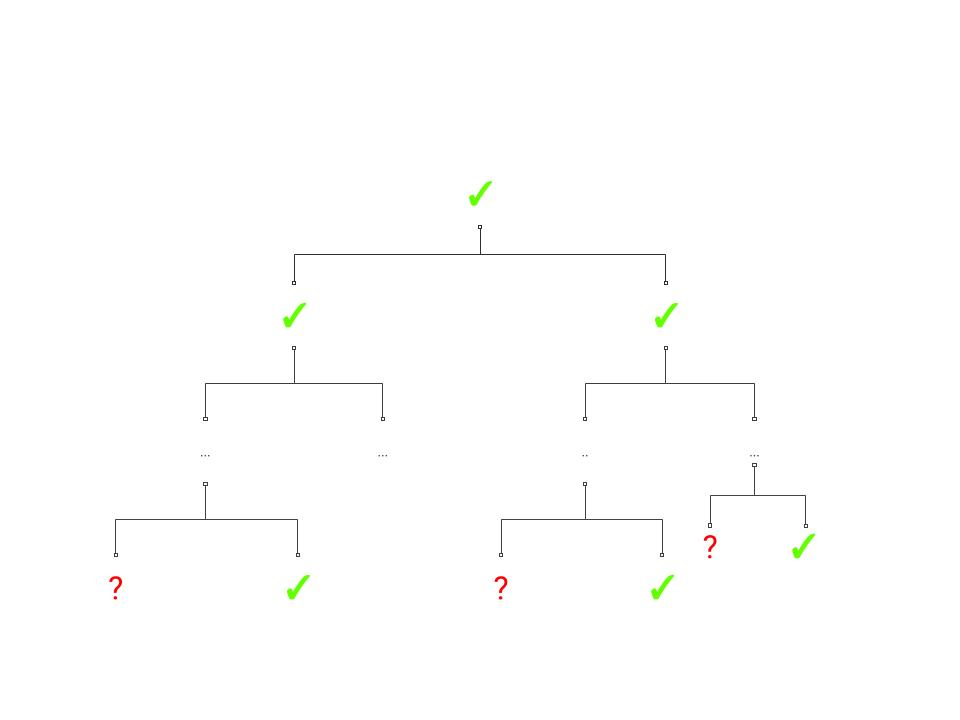
\includegraphics[width=\linewidth, height=1.5in, keepaspectratio]{../figure/Lazy_PRF_from_PRG.jpg}
\caption{In the ``lazy evaluation'' implementation of the black box to
the adversary, we label every node in the tree only when we need it.
Subsequent traversals do not reevaluate the PRG, leading to reuse of the
intermediate seeds. Thus for example, two sibling leaves will correspond
to a single call to \(G(x)\), where \(x\) is their parent's label, but
with the left child receiving the first \(n\) bits and the right child
receiving the second \(n\) bits of \(G(x)\). In this figure check marks
correspond to nodes that have been labeled and question marks to nodes
that are still unlabeled.}
\label{lazyevalprffig}
\end{marginfigure}

Let us consider the ``lazy evaluation'' implementation of the black box
for \(A\) illustrated in \cref{lazyevalprffig}. That is, at every point
in time there are nodes in the full binary tree that are labeled and
nodes which we haven't yet labeled. When \(A\) makes a query \(i\), this
query corresponds to the path \(i_1\ldots i_n\) in the tree. We look at
the lowest (furthest away from the root) node \(v\) on this path which
has been labeled by some value \(y\), and then we continue labelling the
path from \(v\) downwards until we reach \(i\). In other words, we label
the two children of \(v\) by \(G_0(y)\) and \(G_1(y)\), and then if the
path \(i\) involves the first child then we label its children by
\(G_0(G_0(y))\) and \(G_1(G_0(y))\), and so on and so forth (see
\cref{oracleevaltreefig}). Note that because \(G_{0}(y)\) and
\(G_{1}(y)\) correspond to a single call to \(G\), regardless of whether
the traversals continues left or right (i.e.~whether the current level
corresponds to a value 0 or 1 in \(i\)) we label both children at the
same time.


\begin{figure}
\centering
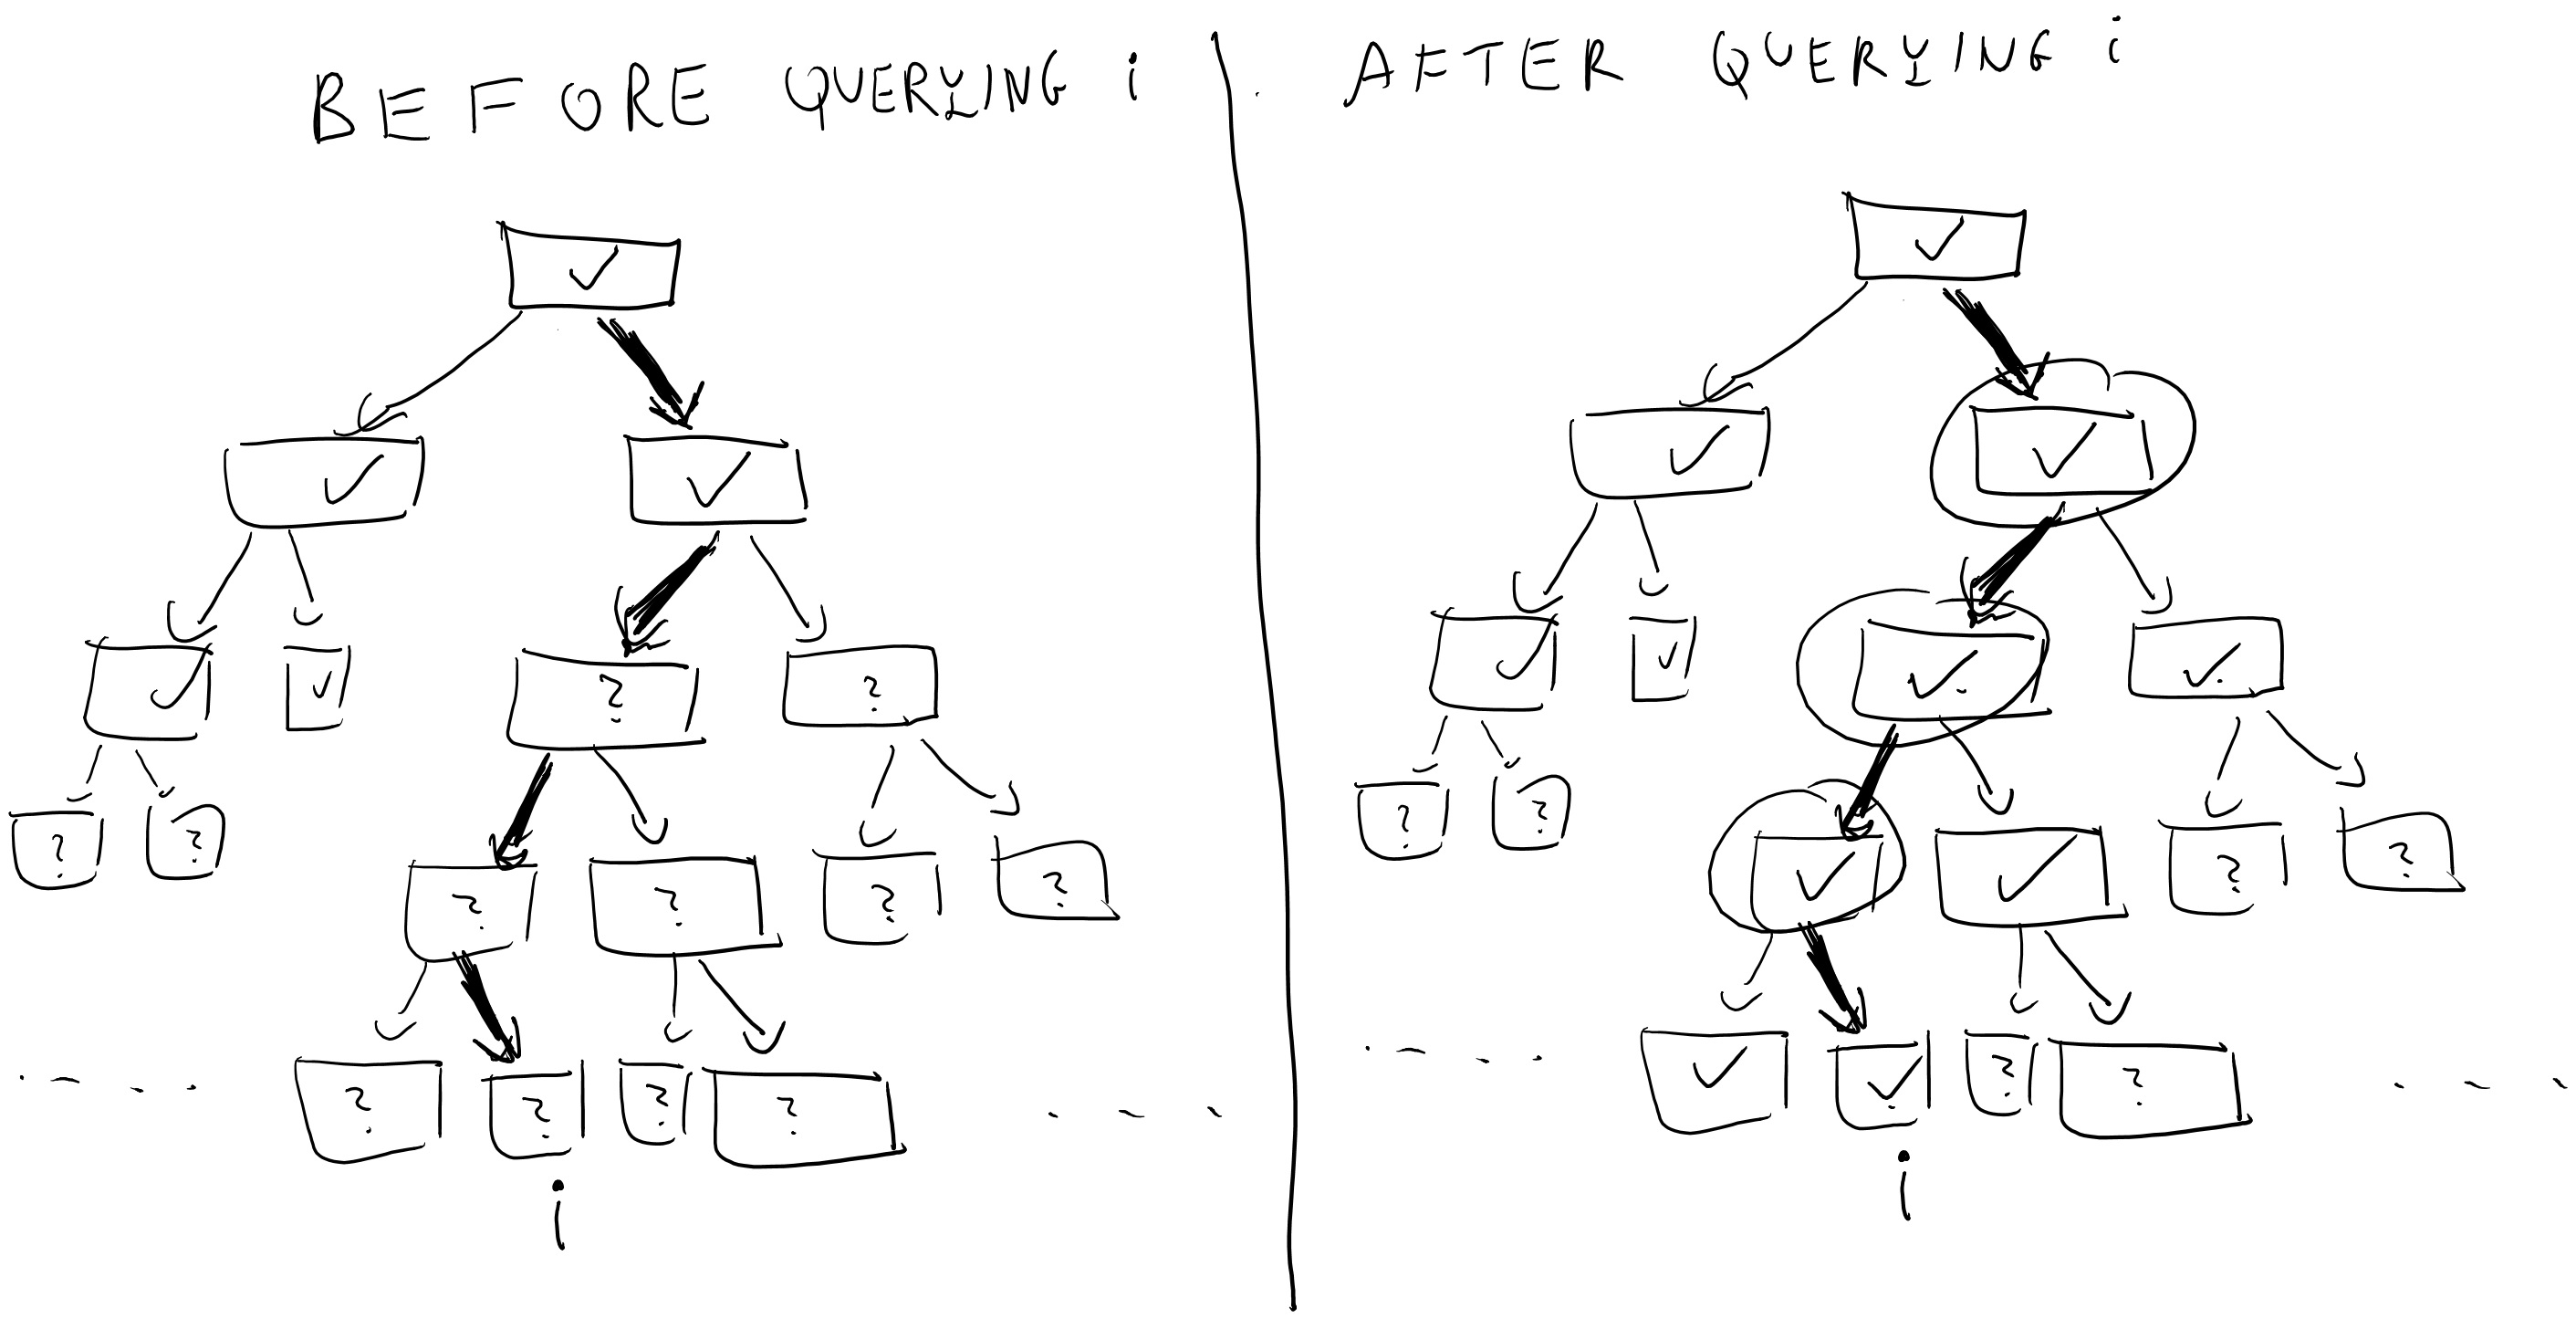
\includegraphics[width=\textwidth, height=0.25\paperheight, keepaspectratio]{../figure/prf-oracle-step.jpg}
\caption{When the adversary queries \(i\), the oracle takes the path
from \(i\) to the root and computes the generator on the minimum number
of internal nodes that is needed to obtain the label of the \(i^{th}\)
leaf.}
\label{oracleevaltreefig}
\end{figure}

A moment's thought shows that this is just another (arguably cumbersome)
way to describe the oracle that simply computes the map
\(i\mapsto f_s(i)\). And so the experiment of running \(A\) with this
oracle produces precisely the same result as running \(A\) with access
to \(f_s(\cdot)\). Note that since \(A\) has running time at most \(T\),
the number of times our oracle will need to label an internal node is at
most \(T' \leq 2nT\) (since we label at most \(2n\) nodes for every
query \(i\)).

We now define the following \(T'\) hybrids: in the \(j^{th}\) hybrid, we
run this experiment but in the first \(j\) times the oracle needs to
label internal nodes, then instead of labelling the \(b^{th}\) child of
\(v\) by \(G_b(y)\) (where \(y\) is the label of \(v\)), the oracle
simply labels it by a random string in \(\{0,1\}^n\).


\begin{figure}
\centering
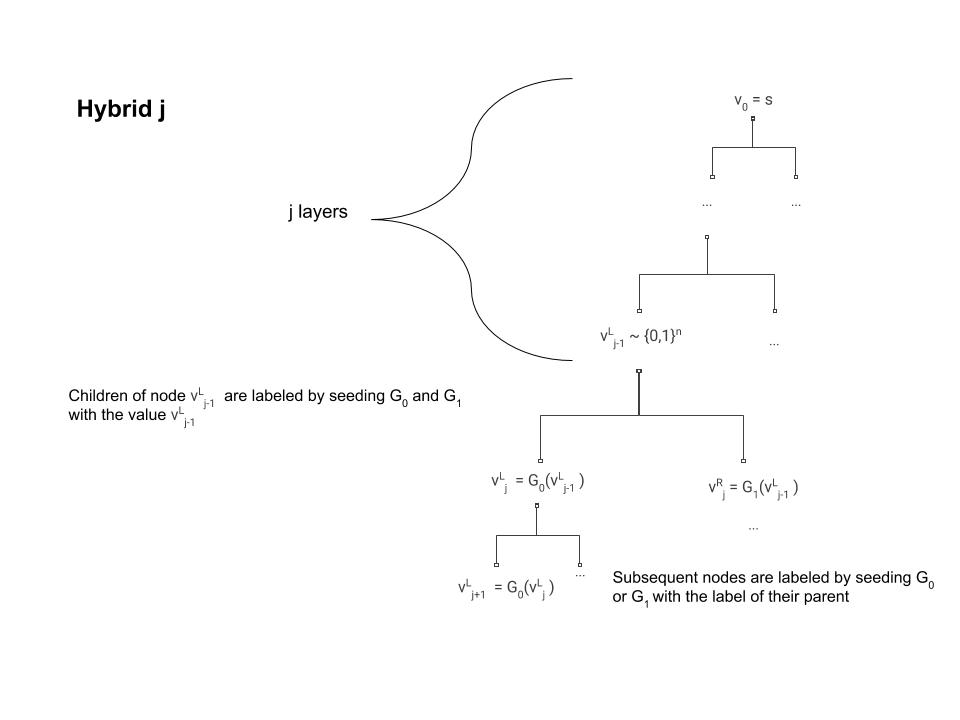
\includegraphics[width=\textwidth, height=0.25\paperheight, keepaspectratio]{../figure/hybrid_j_thm_5-1.jpg}
\caption{In the \(j^{th}\) hybrid all lables up to the first \(j\)
layers of the tree are drawn uniformly at random from \(U_{n}\). All
subsequent children's labels are produced in the usual way by seeding
\(G\) with the label of the parent and assigning the first \(n\) bits
(\(G_{0}\)) to the left child and the last \(n\) bits (\(G_{1}\)) to the
right child. For example, for some node \(v^{L}_{j-1}\) at the
\(j^{th}\) level, we generate pseudorandom string \(G(v^{L}_{j-1})\) and
label the left child \(v^{L}_{j} = G_{0}(v^{L}_{j-1})\) and the right
child \(v^{R}_{j} = G_{1}(v^{L}_{j-1})\). Note that the labeling scheme
for this diagram is different from that in the previous figures. This is
simply for easy of exposition, we could still index our nodes via the
path reaching them from the root.}
\label{hybridj}
\end{figure}


\begin{figure}
\centering
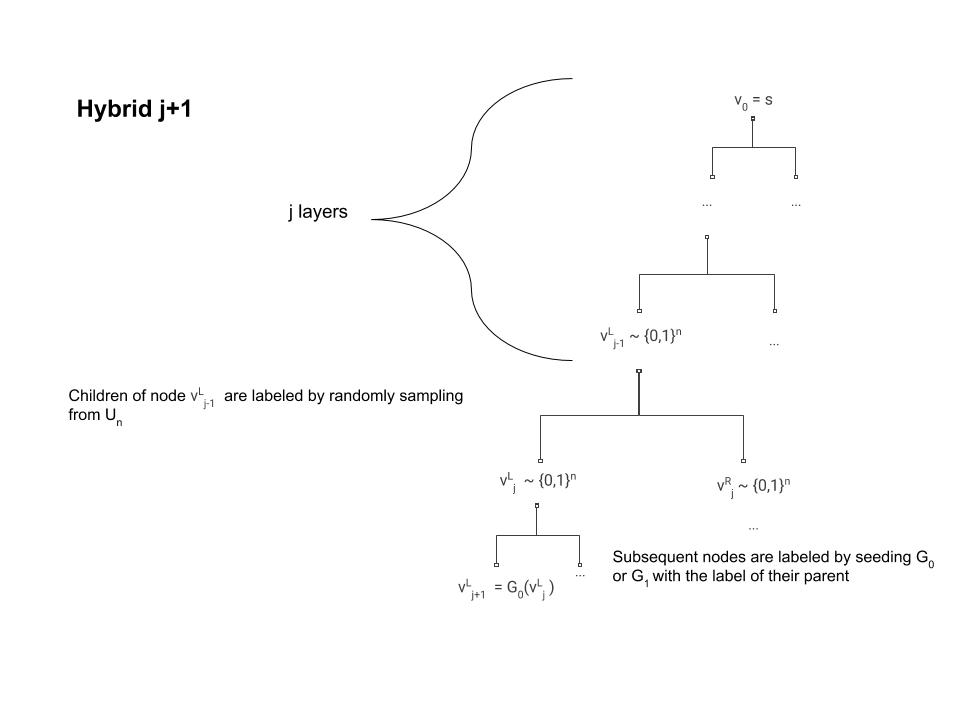
\includegraphics[width=\textwidth, height=0.25\paperheight, keepaspectratio]{../figure/hybrid_j1_thm_5-1.jpg}
\caption{The \(j+1^{st}\) hybrid differs from the \(j^{th}\) in that the
process of assigning random labels continues until the \(j+1^{st}\)
layer of the tree as opposed to the \(j^{th}\). The hybrids are
otherwise completely identically constructed.}
\label{hybridj1}
\end{figure}

Note that the \(0^{th}\) hybrid corresponds to the case where the oracle
implements the function \(i\mapsto f_s(i)\), while in the \(T'^{th}\)
hybrid all labels are random and hence implements a random function. By
the hybrid argument, if \(A\) can distinguish between the \(0^{th}\)
hybrid and the \(T'^{th}\) hybrid with bias \(\epsilon\) then there must
exists some \(j\) such that it distinguishes between the \(j^{th}\)
hybrid (pictured in \cref{hybridj}) and the \(j+1^{st}\) hybrid
(pictured in \cref{hybridj1}) with bias at least \(\epsilon/T'\). We
will use this \(j\) and \(A\) to break the pseudorandom generator.


\begin{figure}
\centering
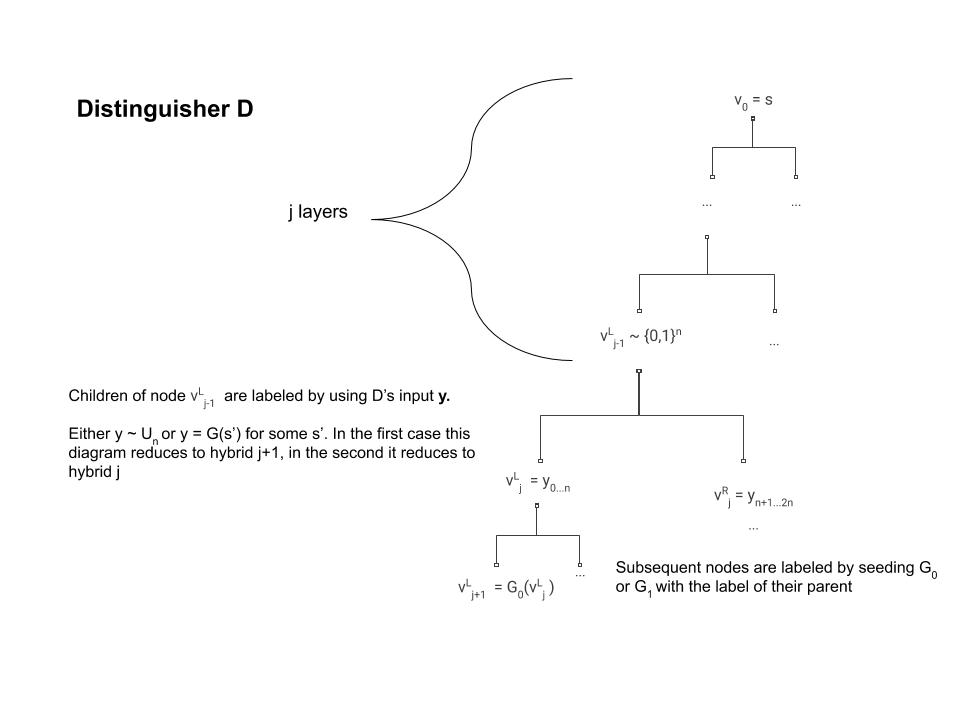
\includegraphics[width=\textwidth, height=0.25\paperheight, keepaspectratio]{../figure/distinguisher_D_thm_5-1.jpg}
\caption{Distinguisher D is similar to hybrid \(j\), in that the nodes
in the first \(j\) layers are assigned completely random labels. When
evaluating along a particular path through \$v\_\{j-1\}\^{}\{L\}, rather
than labeling the two children by applying \(G\) to its label, it simply
splits the input \(y\) into two strings \(y_{0...n}\),\(y_{n+1...2n}\).
If \(y\) is truly random, \(D\) is identical to hybrid \(j+1\). If
\(y=G(s)\) for some random seed \(s\), then \(D\) simulates hybrid
\(j\).}
\label{distinguisherd}
\end{figure}

We can now describe our distinguisher \(D\) (see \cref{distinguisherd})
for the pseudorandom generator. On input a string \(y\in\{0,1\}^{2n}\)
\(D\) will run \(A\) and the \(j^{th}\) oracle inside its belly with one
difference- when the time comes to label the \(j^{th}\) node, instead of
doing this by applying the pseudorandom generator to the label of its
parent \(v\) (which is what should happen in the \(j^{th}\) oracle) it
uses its input \(y\) to label the two children of \(v\).

Now, if \(y\) was completely random then we get exactly the distribution
of the \(j+1^{st}\) oracle, and hence in this case \(D\) simulates
internally the \(j+1^{st}\) hybrid. However, if \(y=G(s)\) for some
randomly sampled \(s\in\{0,1\}^n\), though it may not be obvious at
first, we actually get the distribution of the \(j^{th}\) oracle.

The equivalence between hybrid \(j\) and distinguisher \(D\) under the
condition that \(y=G(s)\) is non obvious, because in hybrid \(j\), the
label for the children of \(v_{j-1}^{L}\) was supposed to be the result
of applying the pseudorandom generator to the label of \(v_{j-1}^{L}\)
and not to some other random string (see \cref{distinguisherd}).
However, because \(v\) was labeled \emph{before} the \(j^{th}\) step
then we know that it was actually labeled by a random string. Moreover,
since we use lazy evaluation we know that step \(j\) is the \emph{first}
time where we actually use the value of the label of \(v\). Hence, if at
this point we \emph{resampled} this label and used a completely
independent random string \(s\) then the distribution of \(v_{j-1}^{L}\)
and \(s\) would be \emph{identical}. Hence the distribution of
\(y=G(s)\), for \(s\) drawn from \(U_n\), is identical to the
distribution, \(G(v_{j-1}^{L}\), of the \(j^{th}\) hybrid, and thus if
\(A\) had advantage \(\epsilon\) in breaking the PRF \(\{ f_s \}\) then
\(D\) will have advantage \(\epsilon/T'\) in breaking the PRG \(G\) thus
obtaining a contradiction.

This proof is ultimately not very hard but is rather confusing. I urge
you to also look at the proof of this theorem as is written in Section
7.5 (pages 265-269) of the KL book.

\end{proof}

\hypertarget{prfpracticerem}{}
\begin{remark}[PRF's in practice] \label[remark]{prfpracticerem}

While this construction reassures us that we can rely on the existence
of pseudorandom functions even on days where we remember to take our
meds, this is not the construction people use when they need a PRF in
practice because it is still somewhat inefficient, making \(n\) calls to
the underlying pseudorandom generators. There are constructions (e.g.,
HMAC) based on hash functions that require stronger assumptions but can
use as few as two calls to the underlying function. We will cover these
constructions when we talk about hash functions and the random oracle
model. One can also obtain practical constructions of PRFs from
\emph{block ciphers}, which we'll see later in this lecture.

\end{remark}

\section{Securely encrypting many messages - chosen plaintext
security}\label{Securely-encrypting-many-}

Let's get back to our favorite task of \emph{encryption}. We seemed to
have nailed down the definition of secure encryption, or did we?

\begin{pause} \label[pause]{Try-to-think-what-kind-of}

Try to think what kind of security guarantees are \emph{not} provided by
the notion of computational secrecy we saw in \cref{compsecdef}

\end{pause}

Our current definition requires talks about encrypting a \emph{single}
message, but this is not how we use encryption in the real world.
Typically, Alice and Bob (or Amazon and Boaz) setup a shared key and
then engage in many back and forth messages between one another. At
first, we might think that this issue of a single long message vs.~many
short ones is merely a technicality. After all, if Alice wants to send a
sequence of messages \((m_1,m_2,\ldots,m_t)\) to Bob, she can simply
treat them as a single long message. Moreover, the way that \emph{stream
ciphers} work, Alice can compute the encryption for the first few bits
of the message she decides what will be the next bits and so she can
send the encryption of \(m_1\) to Bob and later the encryption of
\(m_2\). There is some truth to this sentiment, but there are issues
with using stream ciphers for multiple messages. For Alice and Bob to
encrypt messages in this way, they must maintain a \emph{synchronized
shared state}. If the message \(m_1\) was dropped by the network, then
Bob would not be able to decrypt correctly the encryption of \(m_2\).

There is another way in which treating many messages as a single tuple
is unsatisfactory. In real life, Eve might be able to have some impact
on \emph{what} messages Alice encrypts. For example, the Katz-Lindell
book describes several instances in World War II where Allied forces
made particular military maneuver for the sole purpose of causing the
axis forces to send encryptions of messages of the Allies' choosing. To
consider a more modern example, today Google uses encryption for all of
its search traffic including (for the most part) the \emph{ads} that are
displayed on the page. But this means that an attacker, by paying
Google, can cause it to encrypt arbitrary text of their choosing. This
kind of attack, where Eve \emph{chooses} the message she wants to be
encrypted is called a \emph{chosen plaintext attack}. You might think
that we are already covering this with our current definition that
requires security \emph{for every} pair of messages and so in particular
this pair could chosen by Eve. However, in the case of multiple
messages, we would want to allow Eve to be able to choose \(m_2\)
\emph{after} she saw the encryption of \(m_1\).

All that leads us to the following definition, which is a strengthening
of our definition of computational security:

\hypertarget{cpasecuredef}{}
\begin{definition}[Chosen Plaintext Attack (CPA) secure encryption] \label[definition]{cpasecuredef}

An encryption scheme \((E,D)\) is \emph{secure against chosen plaintext
attack (CPA secure)} if for every polynomial time \(Eve\), Eve wins with
probability at most \(1/2+negl(n)\) in the game defined below:

\begin{enumerate}
\def\labelenumi{\arabic{enumi}.}
\tightlist
\item
  The key \(k\) is chosen at random in \(\{0,1\}^n\) and fixed.\\
\item
  Eve gets the length of the key \(1^n\) as input.\footnote{Giving Eve
    the key as a sequence of \(n\) \(1'\)s as opposed to in binary
    representation is a common notational convention in cryptography. It
    makes no difference except that it makes the input length for Eve of
    length \(n\), which makes sense since we want to allow Eve to run in
    \(poly(n)\) time.}\\
\item
  Eve interacts with \(E\) for \(t=poly(n)\) rounds as follows: in the
  \(i^{th}\) round, Eve chooses a message \(m_i\) and obtains
  \(c_i= E_k(m_i)\).\\
\item
  Then Eve chooses two messages \(m_0,m_1\), and gets \(c^* = E_k(m_b)\)
  for \(b\leftarrow_R\{0,1\}\).\\
\item
  Eve \emph{wins} if she outputs \(b\).\\
\end{enumerate}

\end{definition}


\begin{marginfigure}
\centering
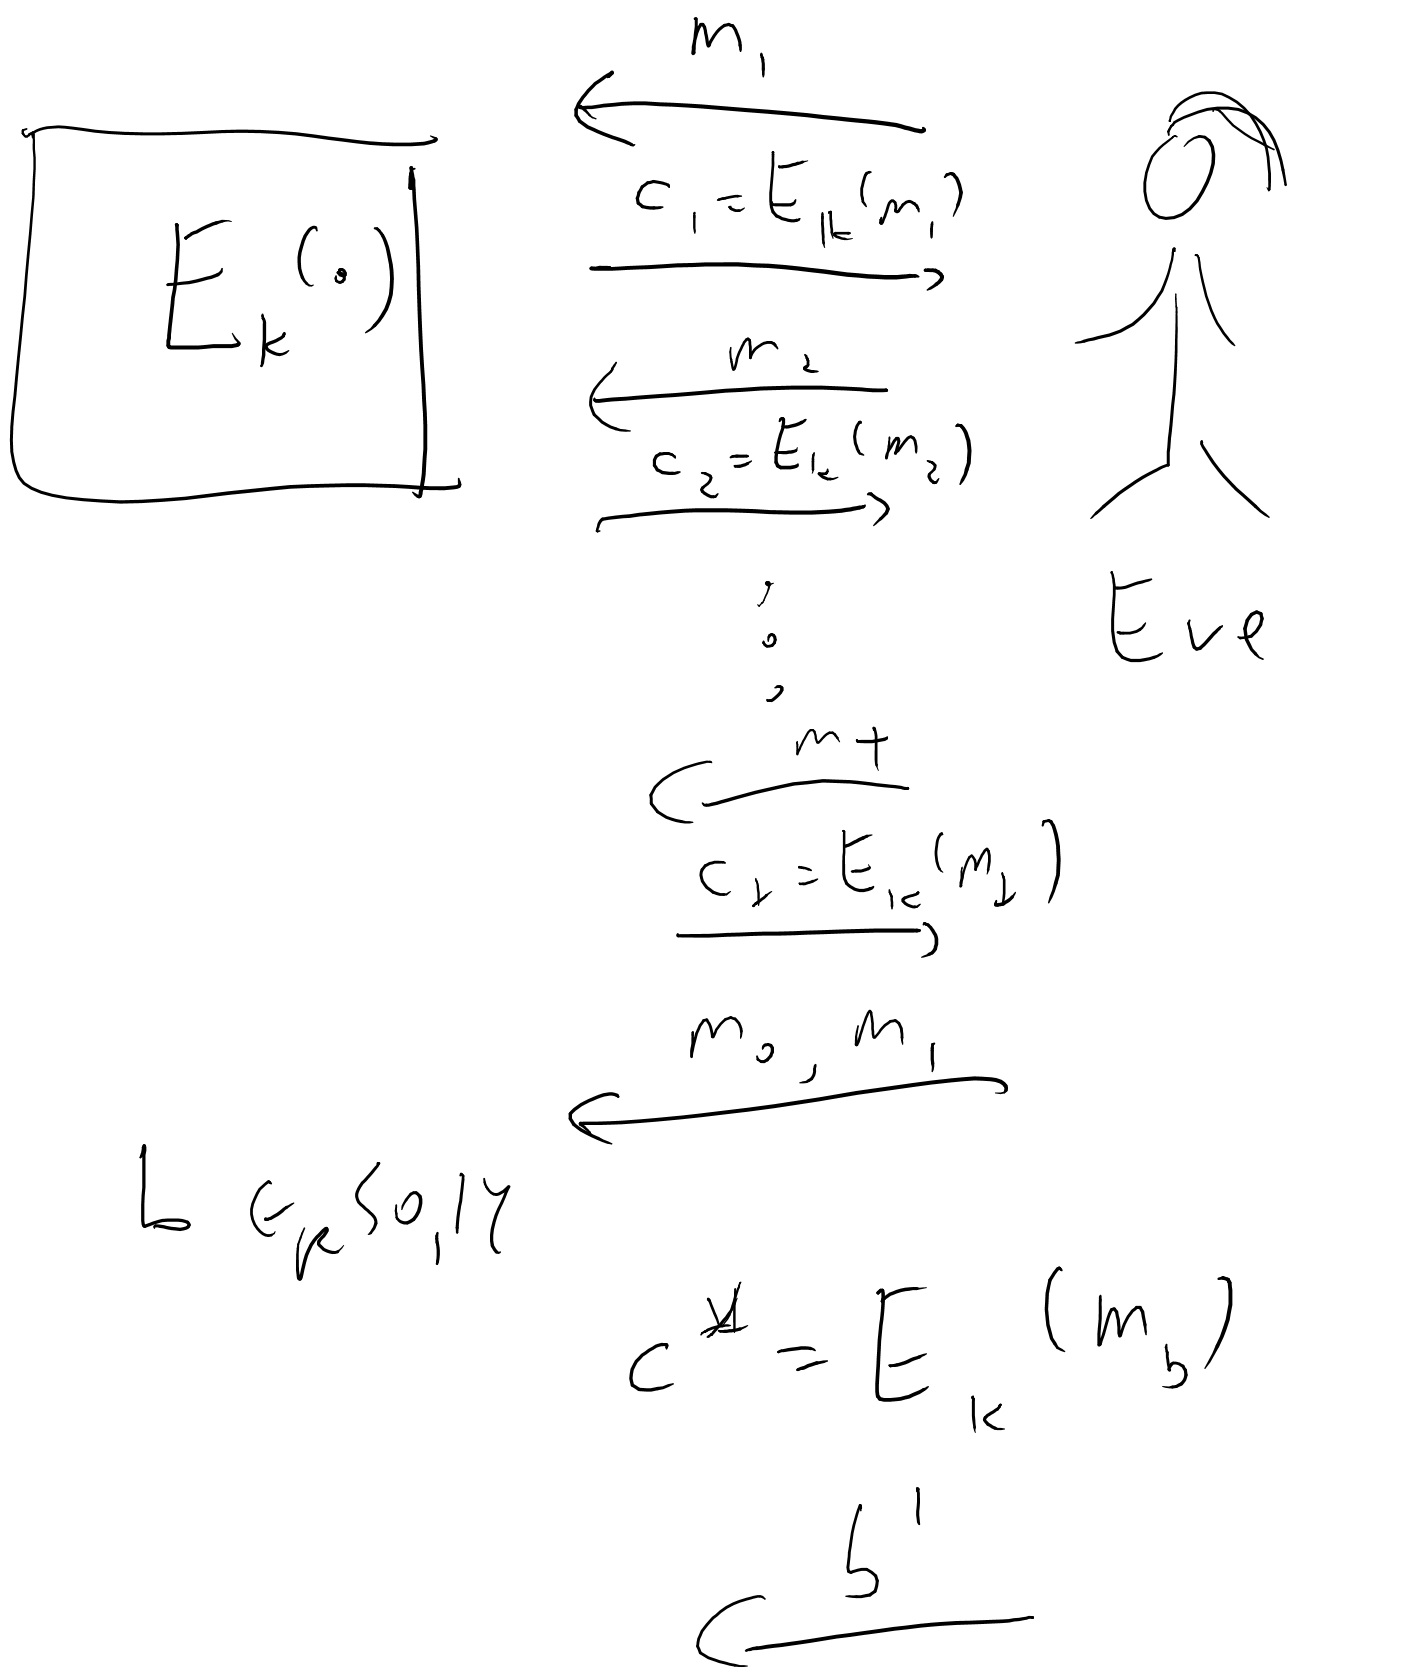
\includegraphics[width=\linewidth, height=1.5in, keepaspectratio]{../figure/cpa-game.jpg}
\caption{In the CPA game, Eve interacts with the encryption oracle and
at the end chooses \(m_0,m_1\), gets an encryption \(c^*=E_k(m_b)\) and
outputs \(b'\). She \emph{wins} if \(b'=b\)}
\label{cpasecgamefig}
\end{marginfigure}

\cref{cpasecuredef} is illustrated in \cref{cpasecgamefig}. Our previous
notion of computational secrecy (i.e., \cref{compsecdef}) corresponds to
the case that we skip Step 3 above. Since Step 3 only gives the
adversary more power (and hence is only more likely to win), CPA
security (\cref{cpasecuredef}) is \emph{stronger} than computational
secrecy (\cref{compsecdef}), in the sense that every CPA secure
encryption \((E,D)\) is also computationally secure. It turns out that
CPA security is \emph{strictly stronger}, in the sense that without
modification, our stream ciphers cannot be CPA secure. In fact, we have
a stronger, and intially somewhat surprising theorem:

\hypertarget{CPAsecrandomthm}{}
\begin{theorem}[CPA security requires randomization] \label[theorem]{CPAsecrandomthm}

There is no CPA secure \((E,D)\) where \(E\) is \emph{deterministic}.

\end{theorem}

\begin{proof} \label[proof]{The-proof-is-very-simple-}

The proof is very simple: Eve will only use a single round of
interacting with \(E\) where she will ask for the encryption \(c_1\) of
\(0^\ell\). In the second round, Eve will choose \(m_0=0^{\ell}\) and
\(m_1=1^{\ell}\), and get \(c^*=E_k(m_b)\) she wil then output \(0\) if
and only if \(c^*=c_1\).

\end{proof}


\begin{marginfigure}
\centering
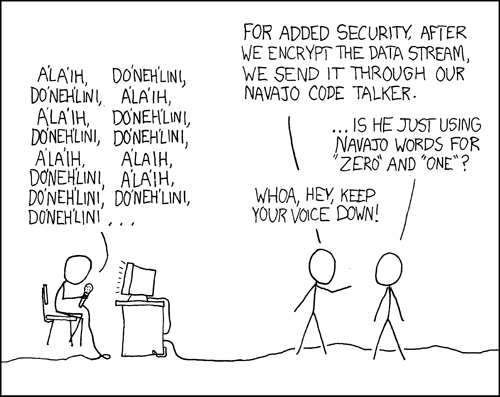
\includegraphics[width=\linewidth, height=1.5in, keepaspectratio]{../figure/code_talkers.png}
\caption{Insecurity of deterministic encryption}
\label{xkcdnavajotwofig}
\end{marginfigure}

This proof is so simple that you might think it shows a problem with the
definition, but it is actually a real problem with security. If you
encrypt many messages and some of them repeat themselves, it is possible
to get significant information by seeing the repetition pattern (que the
XKCD cartoon again, see \cref{xkcdnavajotwofig}). To avoid this issue we
need to use a \emph{randomized} (or \emph{probabilistic}) encryption,
such that if we encrypt the same message twice we \emph{won't} see two
copies of the same ciphertext.\footnote{If the messages are guaranteed
  to have \emph{high entropy} which roughly means that the probability
  that a message repeats itself is negligible, then it is possible to
  have a secure deterministic private-key encryption, and this is
  sometimes used in practice. (Though often some sort of randomization
  or padding is added to ensure this property, hence in effect creating
  a randomized encryption.) Deterministic encryptions can sometimes be
  useful for applications such as efficient queries on encrypted
  databases. See \href{https://goo.gl/GWJLFd}{this lecture} in Dan
  Boneh's coursera course.} But how do we do that? Here pseudorandom
functions come to the rescue:

\hypertarget{cpafromprfthm}{}
\begin{theorem}[CPA security from PRFs] \label[theorem]{cpafromprfthm}

Suppose that \(\{ f_s \}\) is a PRF collection where
\(f_s:\{0,1\}^n\rightarrow\{0,1\}^\ell\), then the following is a CPA
secure encryption scheme: \(E_s(m)=(r,f_s(r)\oplus m)\) and
\(D_s(r,z)=f_s(r)\oplus z\).

\end{theorem}

\begin{proof} \label[proof]{I-leave-to-you-to-verify-}

I leave to you to verify that \(D_s(E_s(m))=m\). We need to show the CPA
security property. As is usual in PRF-based constructions, we first show
that this scheme will be secure if \(f_s\) was an actually random
function, and then use that to derive security.

Consider the game above when played with a completely random function
and let \(r_i\) be the random string chosen by \(E\) in the \(i^{th}\)
round and \(r^*\) the string chosen in the last round. We start with the
following simple but crucial claim:

\textbf{Claim:} The probability that \(r^*=r_i\) for some \(i\) is at
most \(T/2^n\).

\textbf{Proof of claim:} For any particular \(i\), since \(r^*\) is
chosen independently of \(r_i\), the probability that \(r^*=r_i\) is
\(2^{-n}\). Hence the claim follows from the union bound. QED

Given this claim we know that with probability \(1-T/2^n\) (which is
\(1-negl(n)\)), the string \(r^*\) is distinct from any string that was
chosen before. This means that by the lazy evaluation principle, if
\(f_s(\cdot)\) is a completely random function then the value
\(f_s(r^*)\) can be thought of as being chosen at random in the final
round independently of anything that happened before. But then
\(f_s(r^*)\oplus m_b\) amounts to simply using the one-time pad to
encrypt \(m_b\). That is, the distributions \(f_s(r^*)\oplus m_0\) and
\(f_s(r^*)\oplus m_1\) (where we think of \(r^*,m_0,m_1\) as fixed and
the randomness comes from the choice of the random function
\(f_s(\cdot)\)) are both equal to the uniform distribution \(U_n\) over
\(\{0,1\}^n\) and hence Eve gets absolutely no information about \(b\).

This shows that if \(f_s(\cdot)\) was a random function then Eve would
win the game with probability at most \(1/2\). Now if we have some
efficient Eve that wins the game with probability at least
\(1/2+\epsilon\) then we can build an adversary \(A\) for the PRF that
will run this entire game with black box access to \(f_s(\cdot)\) and
will output \(1\) if and only if Eve wins. By the argument above, there
would be a difference of at least \(\epsilon\) in the probability it
outputs \(1\) when \(f_s(\cdot)\) is random vs when it is pseudorandom,
hence contradicting the security property of the PRF.

\end{proof}

\section{Pseudorandom permutations / block
ciphers}\label{Pseudorandom-permutations}

Now that we have pseudorandom functions, we might get greedy and want
such functions with even more magical properties. This is where the
notion of \emph{pseudorandom permutations} comes in.

\hypertarget{PRPdef}{}
\begin{definition}[Pseudorandom permutations] \label[definition]{PRPdef}

Let \(\ell:\N \rightarrow \N\) be some function that is polynomially
bounded (i.e., there are some \(0<c<C\) such that
\(n^c < \ell(n) < n^C\) for every \(n\)). A collection of functions
\(\{ f_s \}\) where \(f_s:\{0,1\}^{\ell} \rightarrow\{0,1\}^{\ell}\) for
\(\ell=\ell(|s|)\) is called a \emph{pseudorandom permutation (PRP)
collection} if:

\begin{enumerate}
\def\labelenumi{\arabic{enumi}.}
\tightlist
\item
  It is a pseudorandom function collection (i.e., the map
  \(s,x \mapsto f_s(x)\) is efficiently computable and there is no
  efficient distinguisher between \(f_s(\cdot)\) with a random \(s\) and
  a random function).\\
\item
  Every function \(f_s\) is a permutation of \(\{0,1\}^\ell\) (i.e., a
  one to one and onto map).\\
\item
  There is an efficient algorithm that on input \(s,y\) returns
  \(f_s^{-1}(y)\).
\end{enumerate}

The parameter \(n\) is known as the \emph{key length} of the
pseudorandom permutation collection and the parameter \(\ell=\ell(n)\)
is known as the \emph{input length} or \emph{block length}. Often,
\(\ell=n\) and so in most cases you can safely ignore this distinction.

\end{definition}

\begin{pause} \label[pause]{At-first-look-crefPRPdef-}

At first look \cref{PRPdef} might seem not to make sense, since on one
hand it requires the map \(x \mapsto f_s(x)\) to be a permutation, but
on the other hand it can be shown that with high probability a random
map \(H:\{0,1\}^\ell \rightarrow \{0,1\}^\ell\) will \emph{not} be a
permutation. How can then such a collection be pseudorandom? The key
insight is that while a random map might not be a permutation, it is not
possible to distinguish with a polynomial number of queries between a
black box that computes a random function and a black box that computes
a random permutation. Understanding why this is the case, and why this
means that \cref{PRPdef} is reasonable, is crucial to getting intuition
to this notion, and so I suggest you pause now and make sure you
understand these points.

\end{pause}

As usual with a new concept, we want to know whether it is possible to
achieve and is useful. The former is established by the following
theorem:

\hypertarget{PRPfromPRF}{}
\begin{theorem}[PRP's from PRFs] \label[theorem]{PRPfromPRF}

If the PRF conjecture holds (and hence by \cref{prfthm} also if the PRG
conjecture holds) then there exists a pseudorandom permutation
collection.

\end{theorem}


\begin{marginfigure}
\centering
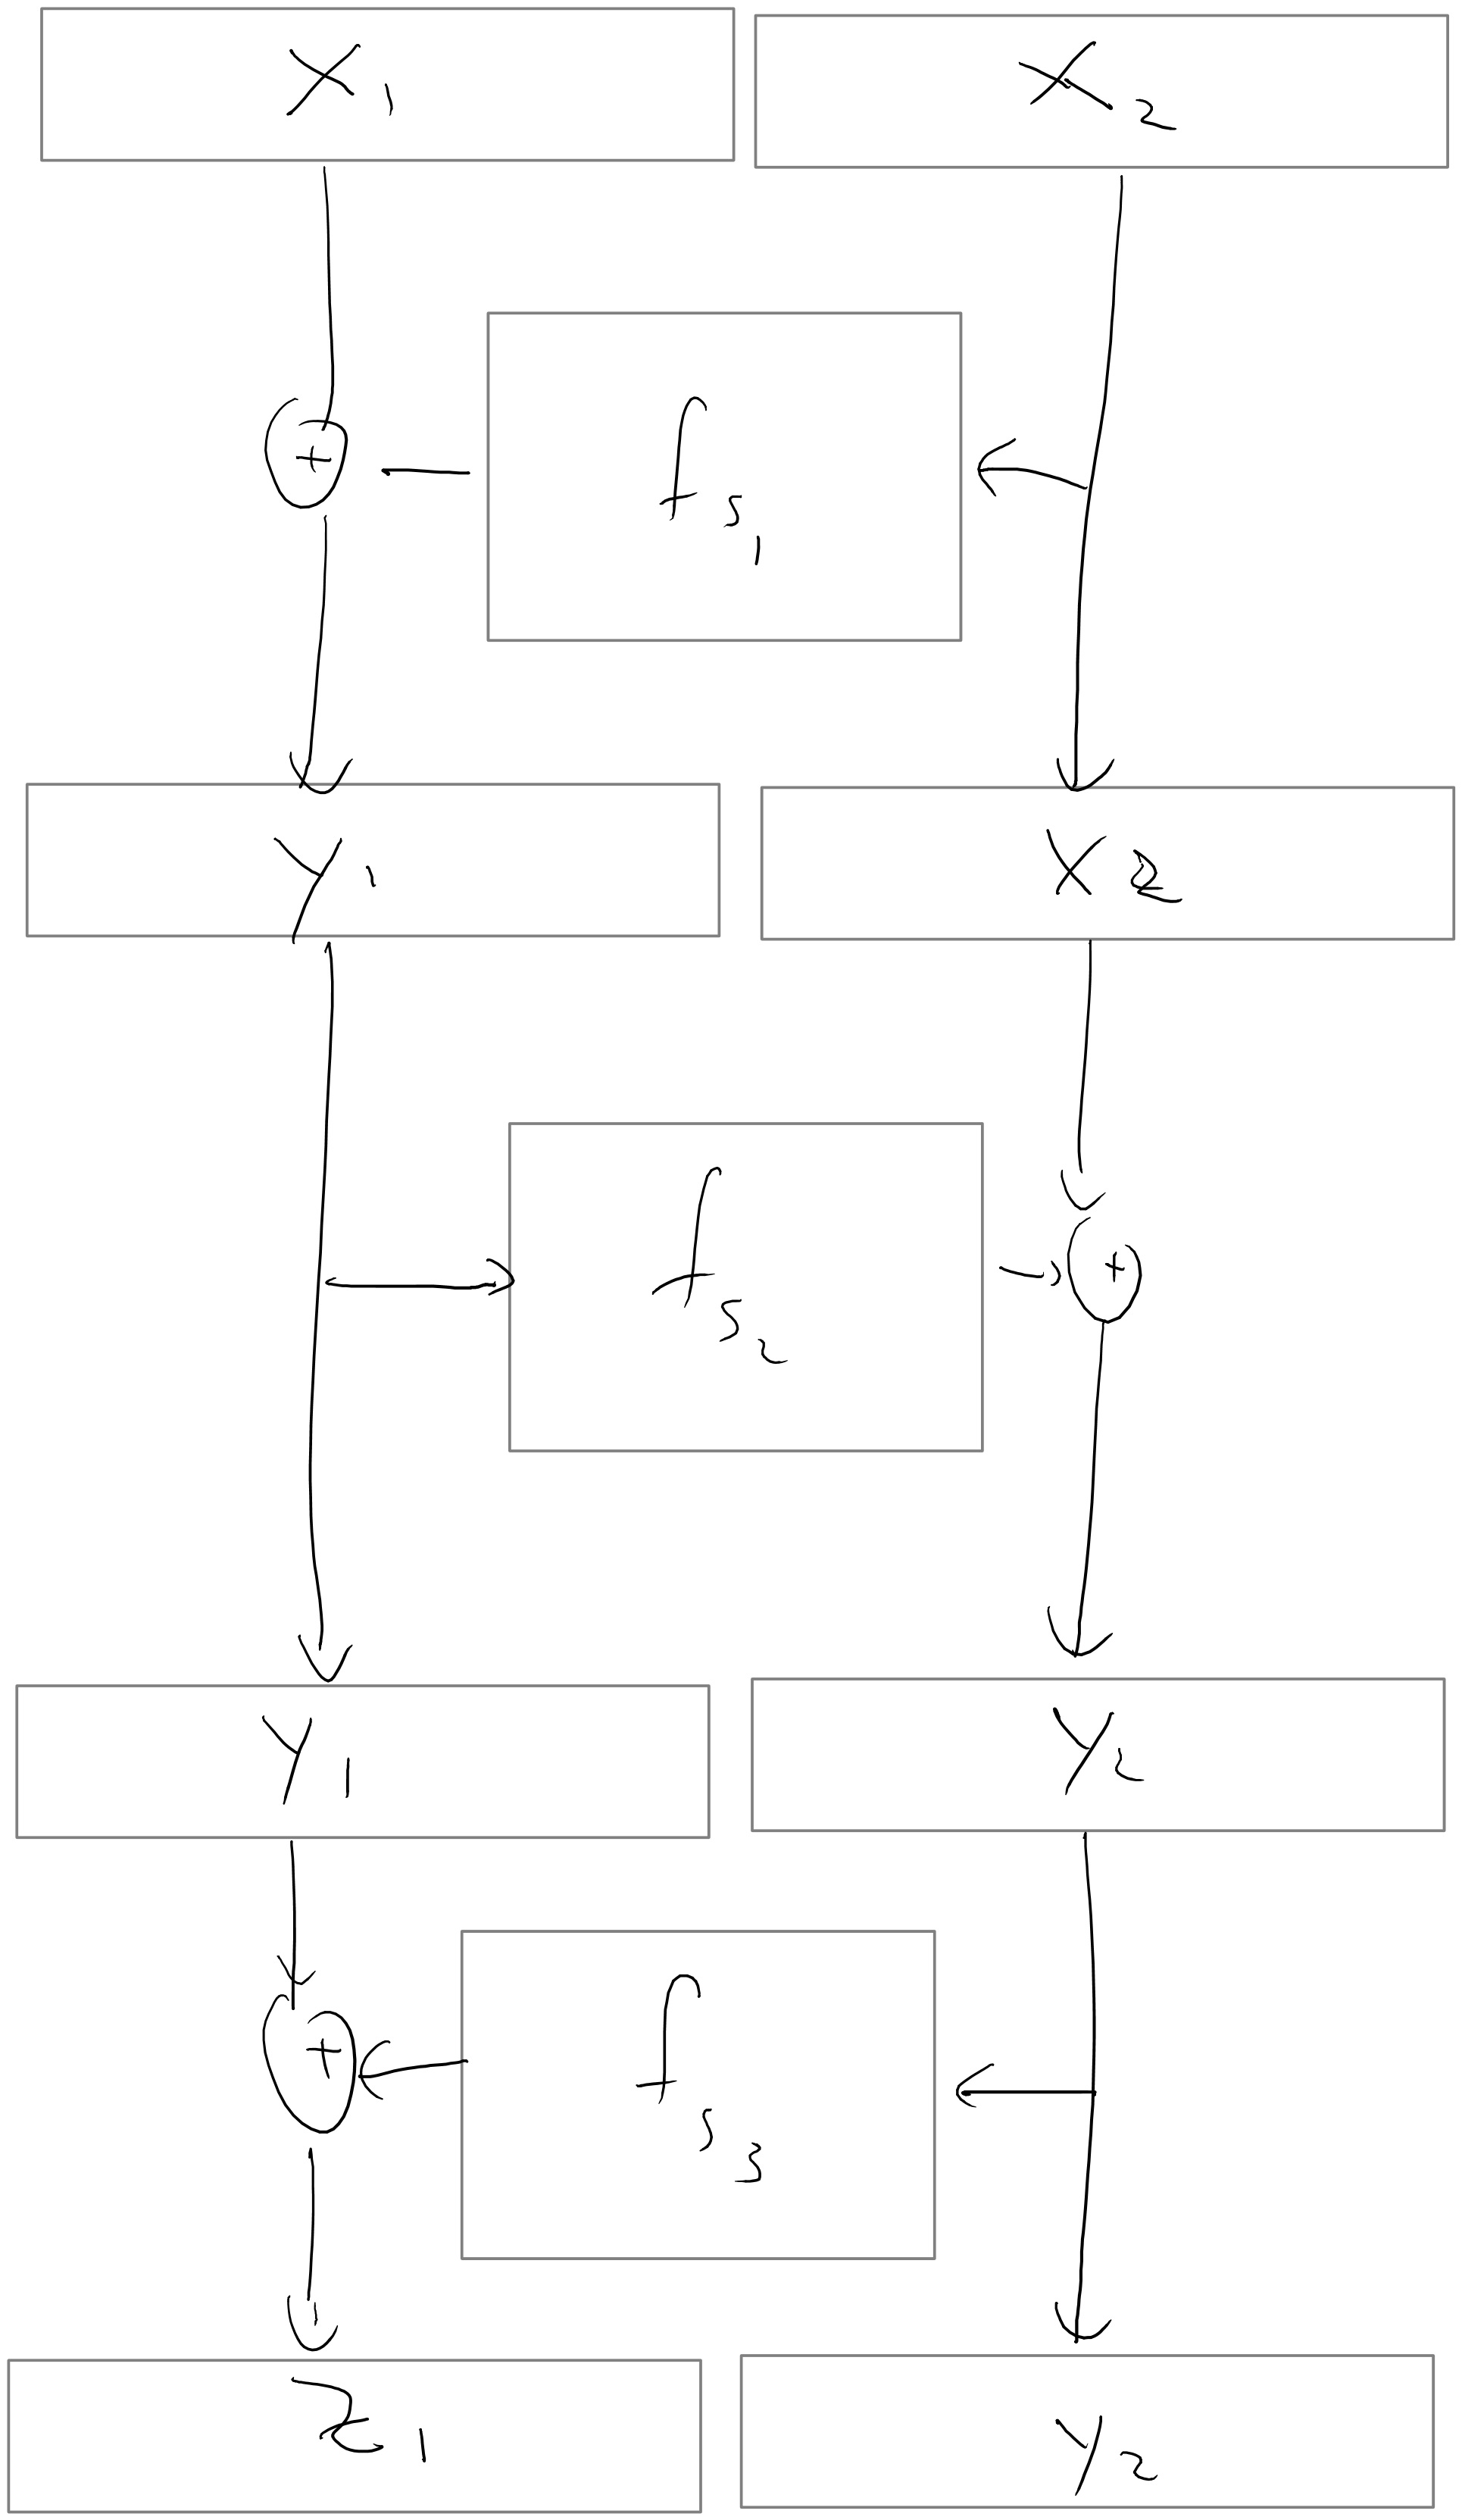
\includegraphics[width=\linewidth, height=1.5in, keepaspectratio]{../figure/feistel.jpg}
\caption{We build a PRP \(p\) on \(2n\) bits from three PRFs
\(f_{s_1},f_{s_2},f_{s_3}\) on \(n\) bits by letting
\(p_{s_1,s_2,s_3}(x_1,x_2)=(z_1,y_2)\) where
\(y_1 = x_1 \oplus f_{s_1}(x_2)\), \(y_2 = x_2 \oplus f_{s_2}(y_1)\) and
\(z_1 = f_{s_3}(y_2) \oplus y_1\).}
\label{feistelfig}
\end{marginfigure}

We will not show the proof of this theorem here, but \cref{feistelfig}
illustrates how the construction of a pseudorandom permutation from a
pseudorandom function looks like. The construction (known as the
Luby-Rackoff construction) uses several rounds of what is known as the
\href{https://en.wikipedia.org/wiki/Feistel_cipher}{Feistel
Transformation} that maps a function
\(f:\{0,1\}^n \rightarrow \{0,1\}^n\) into a permutation
\(g:\{0,1\}^{2n} \rightarrow \{0,1\}^{2n}\) using the map
\((x,y) \mapsto (x,f(x) \oplus y)\). For an overview of the proof see
Section 4.5 in Boneh Shoup or Section 7.6 in Katz-Lindell.

The more common name for a pseudorandom permutation is \emph{block
cipher} (though typically block ciphers are expected to meet additional
security properties on top of being PRPs). The constructions for block
ciphers used in practice don't follow the construction of
\cref{PRPfromPRF} (though they use some of the ideas) but have a more
ad-hoc nature.

One of the first modern block ciphers was the
\href{https://goo.gl/XiCvjs}{Data Encryption Standard (DES)} constructed
by IBM in the 1970's. It is a fairly good cipher- to this day, as far as
we know, it provides a pretty good number of security bits compared to
its key. The trouble is that its key is only \(56\) bits long, which is
no longer outside the reach of modern computing power. (It turns out
that subtle variants of DES are far less secure and fall prey to a
technique known as \href{https://goo.gl/GAvbh8}{differential
cryptanalysis}; the IBM designers of DES were aware of this technique
but kept it secret at the behest of the NSA.)

Between 1997 and 2001, the U.S. national institute of standards (NIST)
ran a competition to replace DES which resulted in the adoption of the
block cipher Rijndael as the new \href{https://goo.gl/1HnqFb}{advanced
encryption standard (AES)}. It has a block size (i.e., input length) of
128 bits and a key size (i.e., seed length) of 128, 196, or 256 bits.

The actual construction of AES (or DES for that matter) is not extremely
illuminating, but let us say a few words about the general principle
behind many block ciphers. They are typically constructed by repeating
one after the other a number of very simple permutations (see
\cref{blockcipherfig}). Each such iteration is called a \emph{round}. If
there are \(t\) rounds, then the key \(k\) is typically expanded into a
longer string, which we think of as a \(t\) tuple of strings
\((k_1,\ldots,k_t)\) via some pseudorandom generator known as the
\emph{key scheduling algorithm}. The \(i\)-th string in the tuple is
known as the \emph{round key} and is used in the \(i^{th}\) round. Each
round is typically composed of several components: there is a ``key
mixing component'' that performs some simple permutation based on the
key (often as simply as XOR'ing the key), there is a ``mixing
component'' that mixes the bits of the block so that bits that were
initially nearby don't stay close to one another, and then there is some
non-linear component (often obtained by applying some simple non-linear
functions known as ``S boxes'' to each small block of the input) that
ensures that the overall cipher will not be an affine function. Each one
of these operations is an easily reversible operations, and hence
decrypting the cipher simply involves running the rounds backwards.


\begin{marginfigure}
\centering
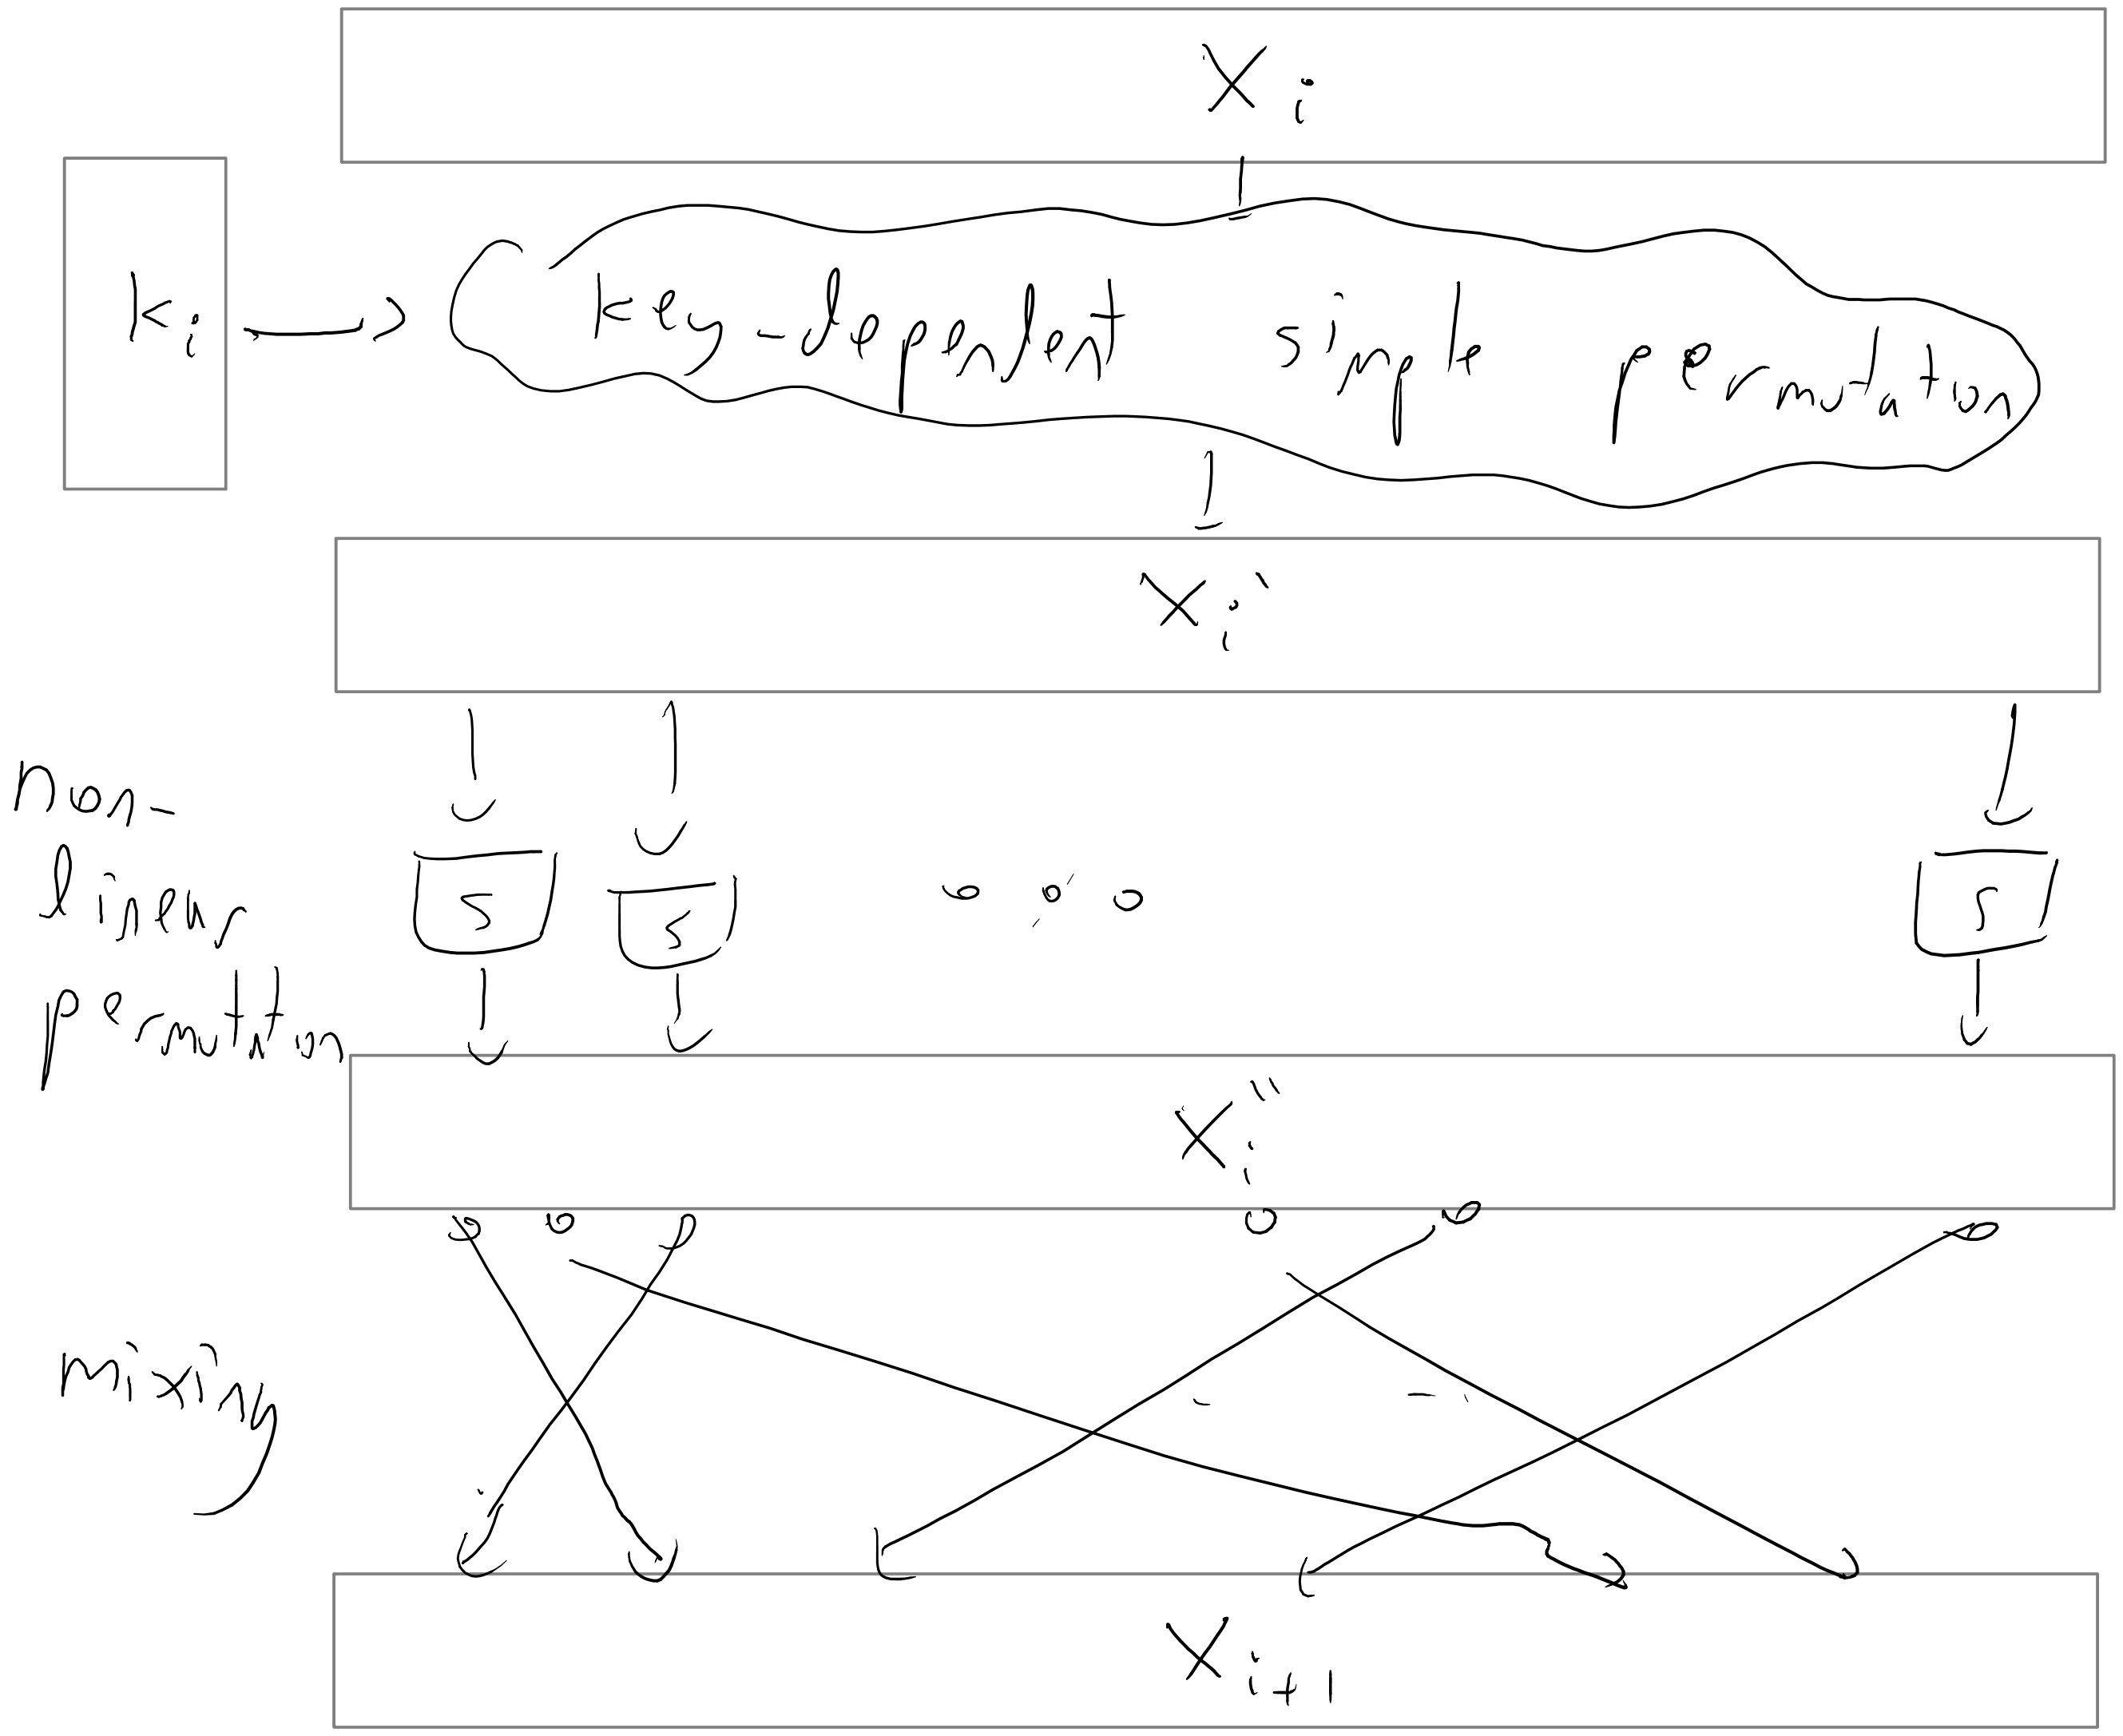
\includegraphics[width=\linewidth, height=1.5in, keepaspectratio]{../figure/block-cipher-round.jpg}
\caption{A typical round of a block cipher, \(k_i\) is the \(^{th}\)
round key, \(x_i\) is the block before the \(i^{th}\) round and
\(x_{i+1}\) is the block at the end of this round.}
\label{blockcipherfig}
\end{marginfigure}

\section{Encryption modes}\label{Encryption-modes}

How do we use a block cipher to actually encrypt traffic? Well we could
use it as a PRF in the construction above, but in practice people use
other ways.\footnote{Partially this is because in the above construction
  we had to encode a plaintext of length \(n\) with a ciphertext of
  length \(2n\) meaning an overhead of 100 percent in the communication.}
The most natural approach would be that to encrypt a message \(m\), we
simply use \(p_s(m)\) where \(\{ p_s \}\) is the PRP/block cipher. This
is known as the \emph{electronic code book (ECB) mode} of a block cipher
(see \cref{ecbonefig}). Note that we can easily decrypt since we can
compute \(p_s^{-1}(m)\). However, this is a \emph{deterministic}
encryption and hence cannot be CPA secure. Moreover, this is actually a
real problem of security on realistic inputs (see \cref{ecbtwofig}).


\begin{marginfigure}
\centering
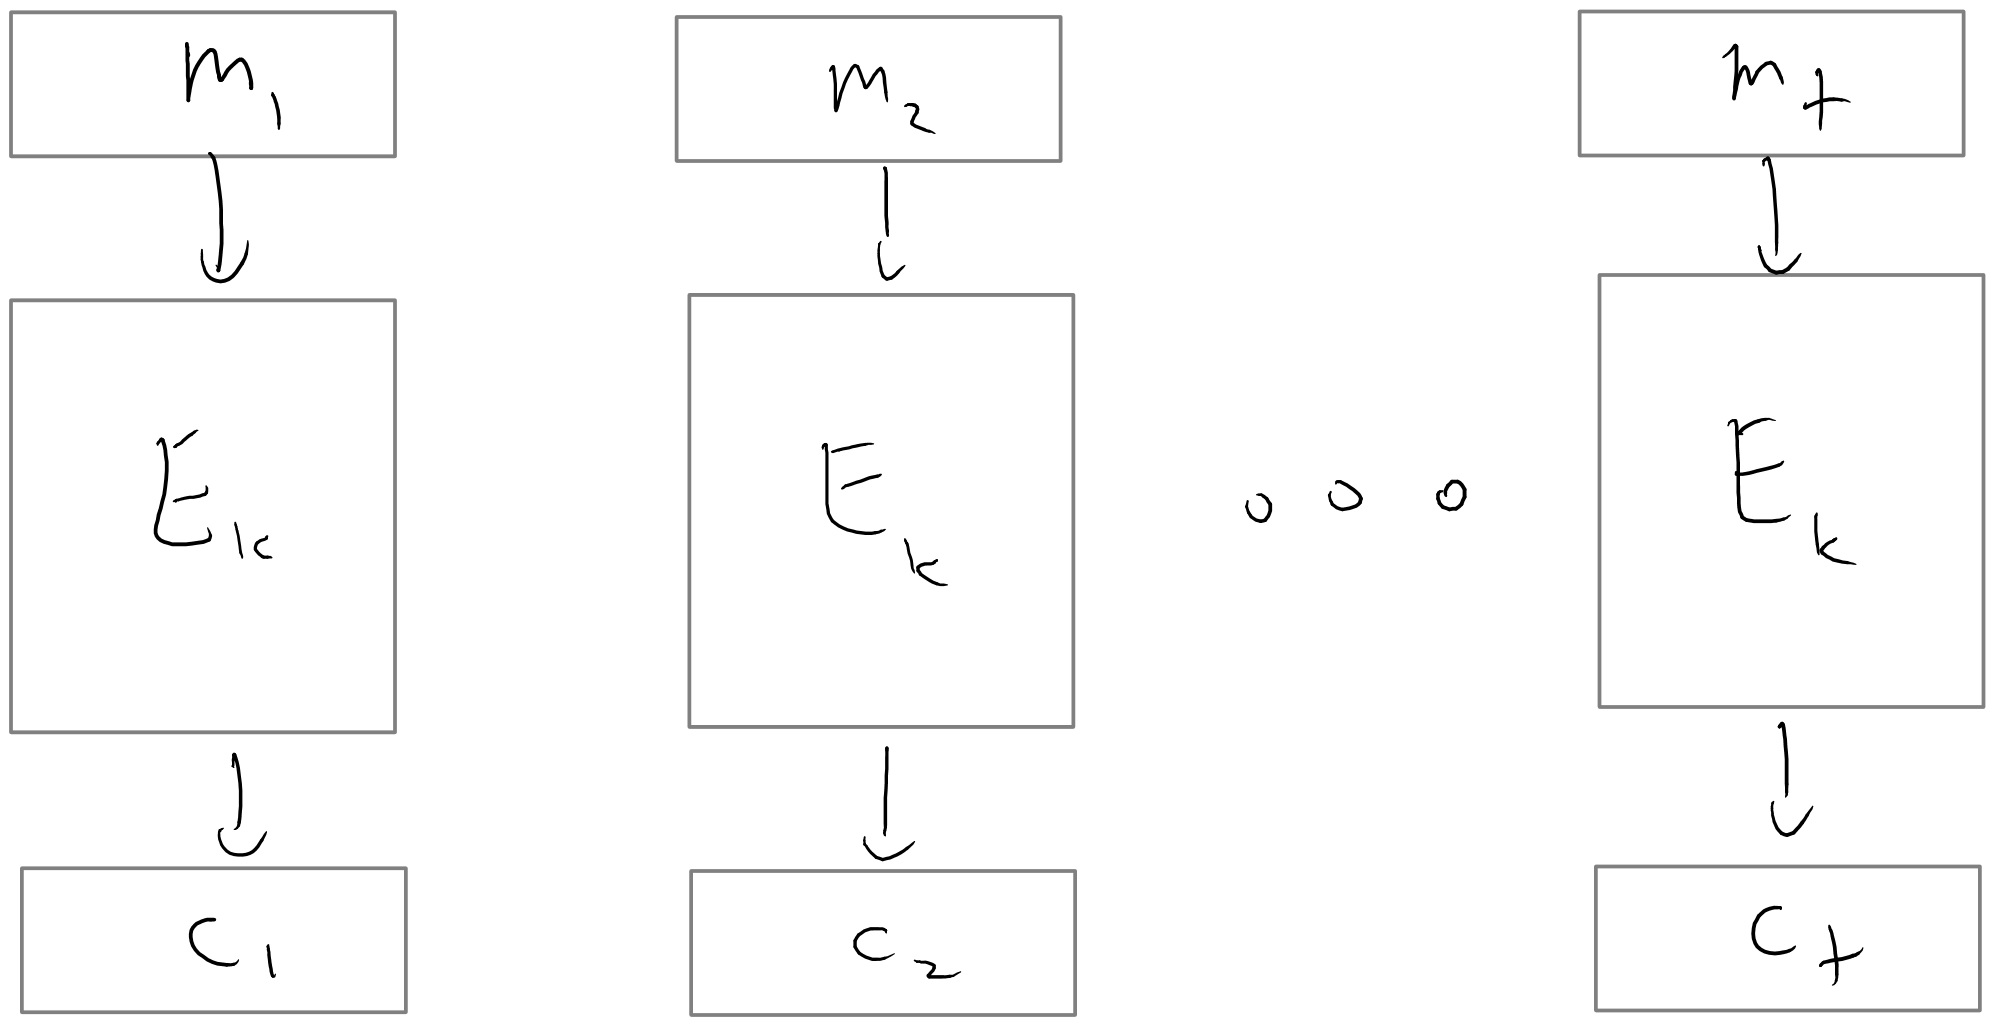
\includegraphics[width=\linewidth, height=1.5in, keepaspectratio]{../figure/ecb-mode.jpg}
\caption{In the Electronic Codebook (ECB) mode every message is
encrypted deterministically and independently}
\label{ecbonefig}
\end{marginfigure}


\begin{marginfigure}
\centering
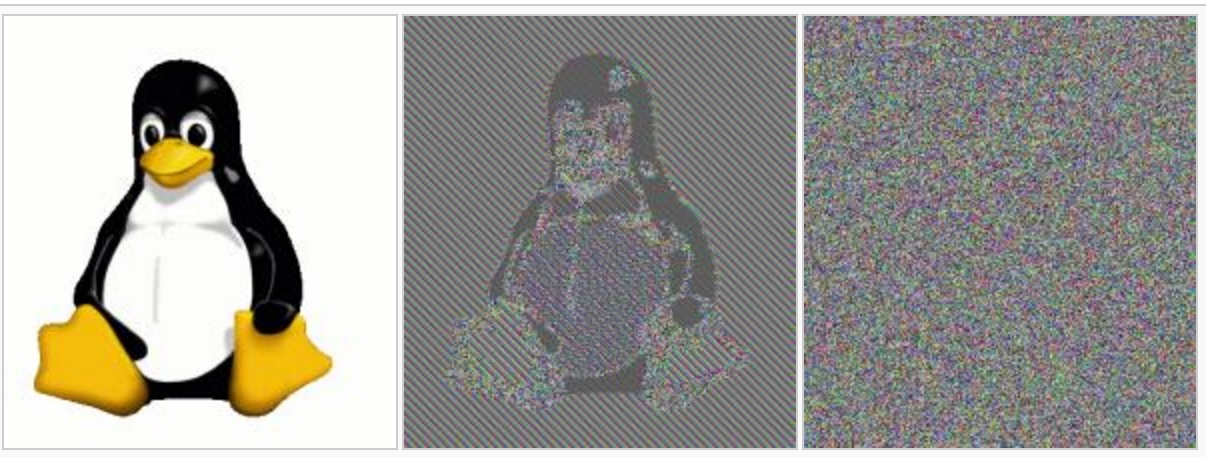
\includegraphics[width=\linewidth, height=1.5in, keepaspectratio]{../figure/ECB_prob.jpg}
\caption{An encryption of the Linux penguin (left image) using ECB mode
(middle image) vs CBC mode (right image). The ECB encryption is insecure
as it reveals much structure about the original image. Image taken from
Wikipedia.}
\label{ecbtwofig}
\end{marginfigure}

A more secure way to use a block cipher to encrypt is the \emph{cipher
block chaining mode} where we XOR every message with the previous
ciphertext (\cref{cbcmodefig}). For the first message we XOR a string
known as the \emph{initialization vector} or IV. Note that if we lose a
block to traffic in the CBC mode then we are unable to decrypt the next
block, but can recover from that point onwards. It turns out that using
this mode with a random IV can yield CPA security, though one has to be
careful in how you go about it, see the exercises.


\begin{marginfigure}
\centering
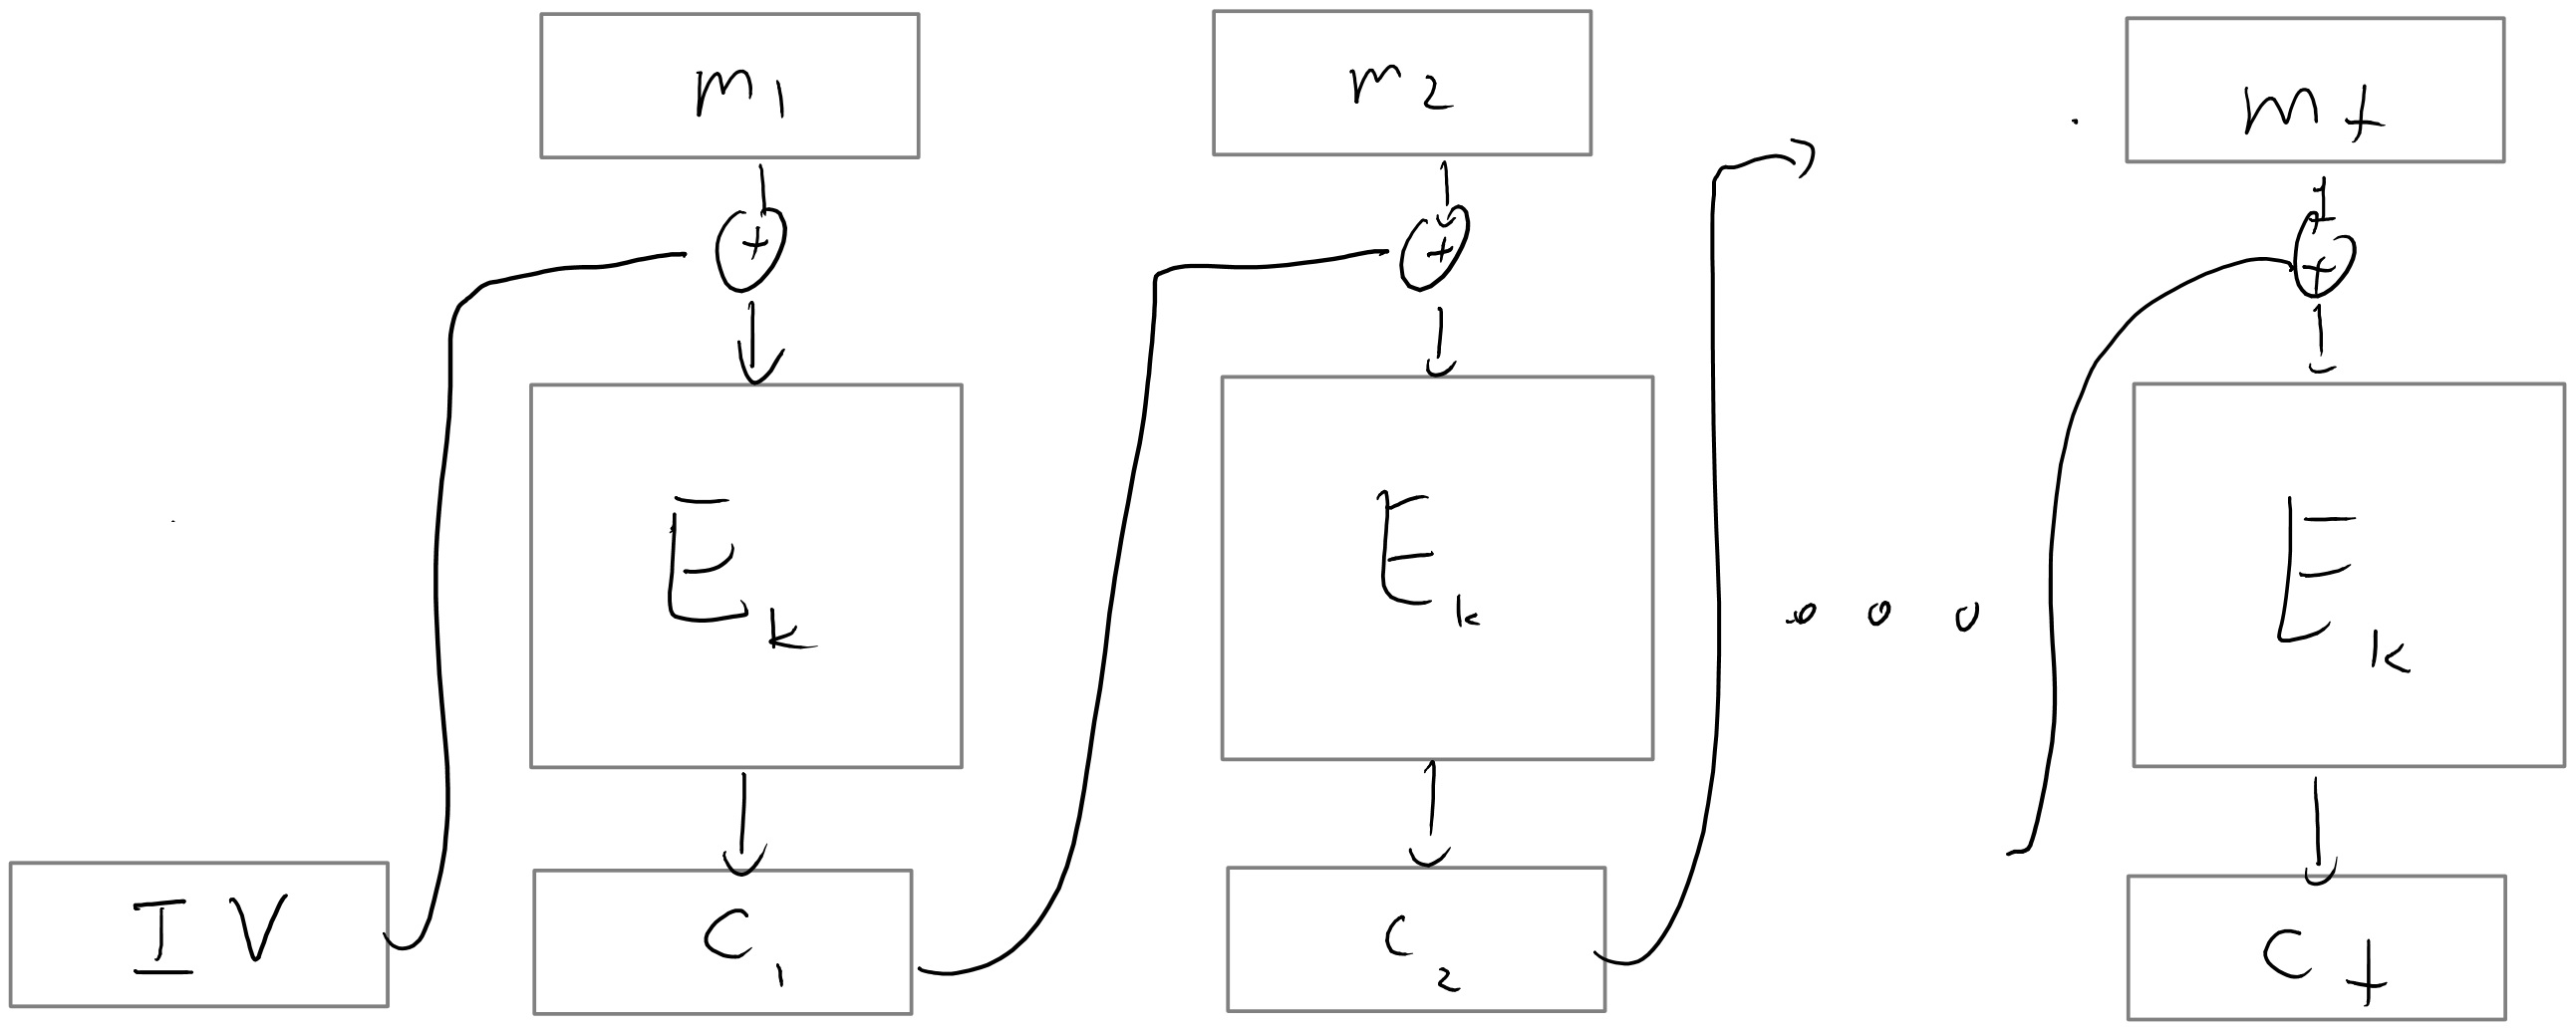
\includegraphics[width=\linewidth, height=1.5in, keepaspectratio]{../figure/cbc-mode.jpg}
\caption{In the Cypher-Block-Chaining (CBC) the encryption of the
previous message is XOR'ed into the current message prior to encrypting.
The first message is XOR'ed with an \emph{initialization vector} (IV)
that if chosen randomly, ensures CPA security.}
\label{cbcmodefig}
\end{marginfigure}

In the \emph{output feedback mode (OFB)} we encrypt the all zero string
using CBC mode to get a sequence \((y_1,y_2,\ldots)\) of pseudorandom
outputs that we can use as a stream cipher. Perhaps the simplest mode is
\emph{counter mode} where we convert a block cipher to a stream cipher
by using the stream
\(p_k(\ensuremath{\mathit{IV}}),p_k(\ensuremath{\mathit{IV}}+1),p_k(\ensuremath{\mathit{IV}}+2),\ldots\)
where \(\ensuremath{\mathit{IV}}\) is a random string in \(\{0,1\}^n\)
which we identify with \([2^n]\) (and perform addition modulo \(2^n\)) .
For a modern block cipher this should be no less secure than CBC or OFB
and has advantages that we can easily compute it in parallel.

A fairly comprehensive study of the different modes of block ciphers is
in \href{http://web.cs.ucdavis.edu/~rogaway/papers/modes.pdf}{this
document by Rogaway}. His conclusion is that if we simply consider CPA
security (as opposed to the stronger notions of \emph{chosen ciphertext
security} we'll see in the next lecture) then counter mode is the best
choice, but CBC, OFB and CFB are widely implemented due to legacy
reasons. ECB should not be used (except as a building block as part of a
construction achieving stronger security).
